\section{气体、液体和固体的分子结构}\label{sec:5-2}

我们知道,气体既没有一定的体积,又没有一定的形状;
液体有一定的体积,但没有一定的形状;
固体既有一定的体积,又有一定的形状。
气体、液体和固体的这种区别,可以用它们的分子结构的不同来说明。

\begin{wrapfigure}{r}{6cm}
    \centering
    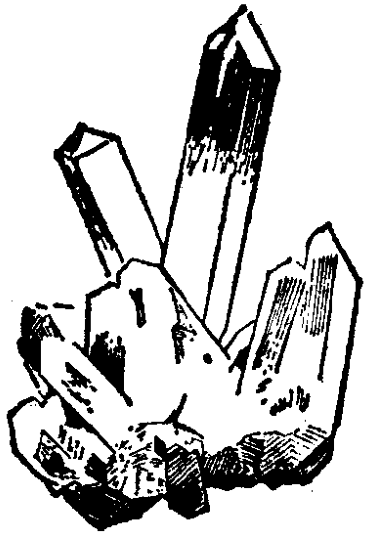
\includegraphics[width=5cm]{../pic/czwl2-ch5-3}
    \caption{水晶}\label{fig:5-3}
\end{wrapfigure}

\xiaobiaoti{气体}
气体很容易被压缩,说明气体分子间的距离比较大,在 0 ℃ 和 1 标准大气压下,
气体分子间的距离大约是分子直径的 10 倍。
这时分子间的作用力很小,可以近似地认为,气体分子除了相互碰撞或跟器壁碰撞外是不受作用力的。
所以,气体分子在没有跟别的分子或器壁碰撞时做匀速直线运动,只有受到碰撞时才改变速度的大小和方向。
由于气体分子的数目很大,分子间的相互碰撞十分频繁。整个看来,气体分子在做杂乱无章的运动。
由于气体分子可以在空间里到处移动,因此气体能充满它所能达到的空间,没有一定的体积,也没有一定的形状。

\xiaobiaoti{固体}
固体分子间的距离很小,只有几个埃,它们间的作用力很大,
绝大多数的分子只能在各自的平衡位置附近做无规则的振动。
正是由于这样,固体才能保持一定的体积和形状。

我们已经知道,固体分晶体和非晶体两类。
晶体的分子的排列是有规则的。因此晶体具有规则的天然形状。
图 \ref{fig:5-3} 是天然水晶的外形。
非晶体的分子的排列没有规则,因此非晶体没有规则的天然形状。

晶体又可分为单晶体和多晶体两类。
物体的分子按统一的规则排列成一个大晶体的,叫做单晶体。食盐、水晶等的单个晶体就是单晶体。
如果物体是由许多杂乱无章的小晶粒构成的,每个晶粒虽然有规则的外形,
但整个物体却没有规则的外形,这种晶体就叫做多晶体。常见的金属都是多晶体。

\xiaobiaoti{液体}
液体的分子结构介于气体和固体之间。
液变成气体时,体积增大一千倍左右,
变成固体时,体积变化不大,可见液体的分子结构比较接近于固体。

液体分子间的作用力比固体的小,分子的排列没有一定的规则,
液体分子也象固体分子那样在平衡位置附近做无规则的振动,
不过振动一段短时间后,就移动到别的位置,再振动一段时间后,又移动到别的位置。
正是由于液体分子运动的这个特点,使液体容易流动,没有一定的形状。
但液体分子间的距离也比较小,因此不易被压缩,而有一定的体积。

知道了气体、液体和固体的分子结构,就不难用分子运动论的知识来解释物态变化了。
例如,晶体的分子的排列是有规则的,在温度升高时,分子的振动加剧,
温度升高到一定程度,分子间的相互作用力已不能把分子限制在平衡位置附近振动,
于是有规则的排列被破坏,固体变为液体,这就是熔解。
不停地做无规则运动的液体分子中,总有一些分子的速度大到能够克服液面其他分子的吸引,
跑到液体外面去,成为气体分子,液体变为气体,这就是蒸发。


\lianxi

(1) 1 克蔗糖含有 $1.8 \times 10^{21}$ 个分子。把 1 克蔗糖放到蓄水 $10^{10} \lfm$ 的大水库中,
如果蔗糖分子均匀分布到整个水库中,每立方厘米的水中含有多少个蔗糖分子?

(2) 算算看,一个水分子的质量是多大?

(3) 撒一些粗盐块到一杯水里,过些时候,盐块看不见了,全杯水都变咸了。为什么?


